\documentclass[7pt,a4paper]{article}

\usepackage{graphicx}
\usepackage{sectsty}

\sectionfont{\fontsize{10}{11}\selectfont}
\subsectionfont{\fontsize{10}{11}\selectfont}

\begin{document}
\textbf{\LARGE Assignment 2b Report - Text Mining}
\section{Introduction}
Given a collection of text documents we aim to find similar documents. In order to do that we normalized the text and created a Tf-idf matrix of collection and used cosine similarity to create a similarity matrix. Also applied K-means clustering and hierarchical clustering in order to identify clusters of similar documents.

\section{Packages Used - \textit{(Language: Python)}}
\begin{itemize}
\item{\textbf{Sklearn}:Package used for constructing Tf-idf, cosine similarity and for K-means}
\item{\textbf{NLTK}: Package used for Natural Language Processing.}
\item{\textbf{Scipy}: Package which provides function for plotting dendogram and linkage for Hierarchical Clustering.}
\item{\textbf{Seaborn}: Used for visualization of data through plots}
\item{\textbf{Matplotlib}: Used for plotting of graphs}
\item{\textbf{Pandas}: Package which provides Data structure like DataFrame which makes
manipulation of datasets easy}
\end{itemize}

\section{Dataset}
Twenty two text documents were taken all being on the Topic- \textbf{‘The History of web search engines’}. Texts are preprocessed and consists of terms for each document. 

\section{Methods and Observations}

\subsection{Tf-idf}

\subsection{K-means}

\subsection{Cosine similarity}
\begin{figure}[h]
\centering
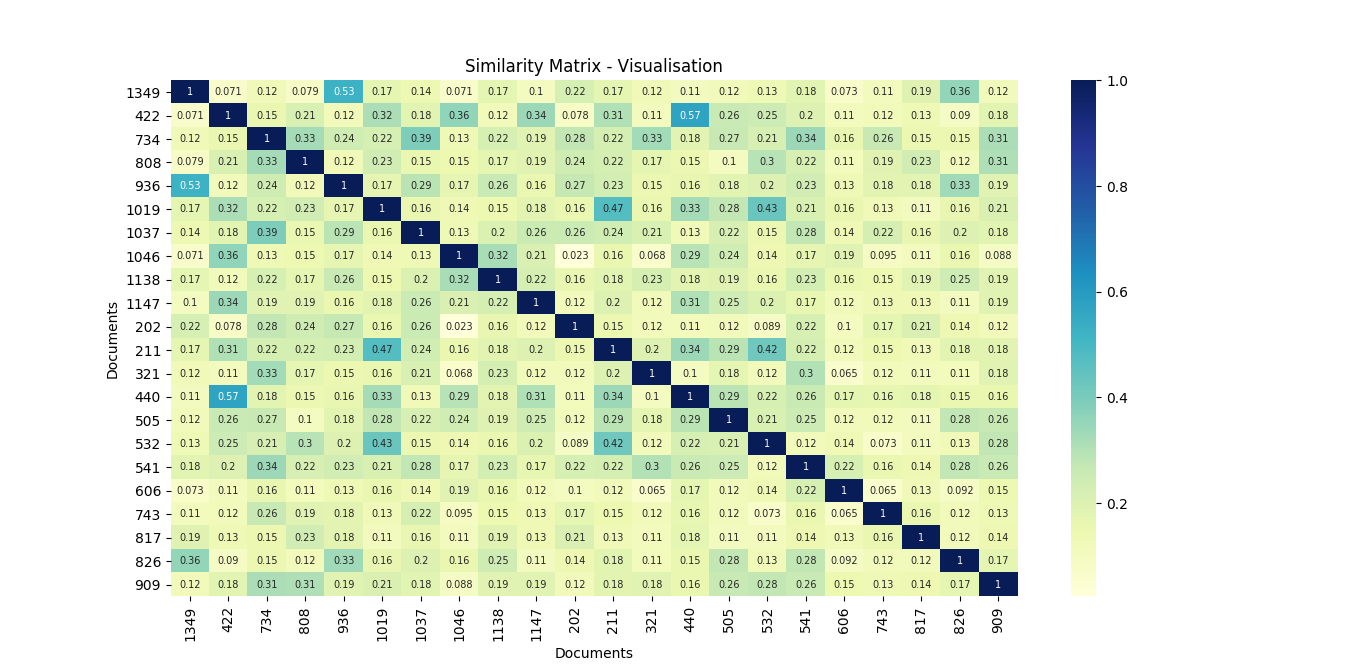
\includegraphics[scale=.40]{similarity1b}
\caption{Similarity matrix - Cosine Similarity}
\label{image-J-C}
\end{figure}


\subsection{Hierarchical Clustering}
\begin{itemize}
\item{\textbf{Distance matrix}: It is obtained by calculating \textit{(1-Cosine Similarity)} between each pair of the documents}
\item{\textbf{Linkage Parameter} : Single Linkage}
\item{Dendogram is shown in the figure \ref{image-Dendogram} below where the horizontal axis represents the pairwise dissimilarity between documents}
\end{itemize}



\end{document}
